\begin{frame}{A 50-50 split slide}

  \begin{columns}
    \begin{column}{0.5\linewidth}
      \begin{itemize}
        \item This side has a bullet
        \item And another bullet, with text that wraps if it's long
      \end{itemize}
    \end{column}
    \begin{column}{0.5\linewidth}
      \begin{figure}
        \centering
        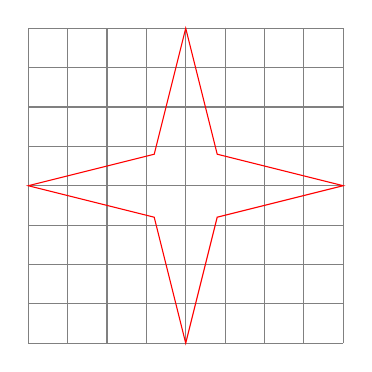
\begin{tikzpicture}[scale=2]
          \draw[step=0.25cm,color=gray] (-1,-1) grid (1,1);
          \draw[color=red] (1,0) -- (0.2,0.2) -- (0,1) -- (-0.2,0.2) -- (-1,0)
          -- (-0.2,-0.2) -- (0,-1) -- (0.2,-0.2) -- cycle;
        \end{tikzpicture}
        \caption{A figure caption}
      \end{figure}
    \end{column}
  \end{columns}

  \note{
    This slide has notes too.
  }

\end{frame}
